\documentclass[9pt,portrait]{article}
\usepackage{beamerarticle} % makes slides into article

%% xcolor Option Clash issue
%	Do not include xcolor,, tikz-qtree, todonotes, here do it after beamerarticle
\usepackage{multicol}
\usepackage{booktabs}
\usepackage{calc}
\usepackage{ifthen}
\usepackage[portrait]{geometry}
\usepackage{hyperref}
\usepackage{color}
\usepackage{enumitem}
\usepackage{textcomp} 				% copyleft symbol
\usepackage{verbatim}
\usepackage{adjustbox} 				% for resizebox to adjust table figure content
\usepackage{enumitem}				% margin free lists
\usepackage{amsmath}
\usepackage{mathrsfs}
\usepackage{csvsimple}				% importing csv as table
\usepackage{textcomp} 				% copyleft symbol
\usepackage{graphicx}
\usepackage{etoolbox} % conditional inclusions

\usepackage{media9}
 \usepackage{multimedia}
 \usepackage{makecell}
 \usepackage{listings}
%  \usepackage{color}
 
\definecolor{codegreen}{rgb}{0,0.6,0}
\definecolor{codegray}{rgb}{0.5,0.5,0.5}
\definecolor{codepurple}{rgb}{0.58,0,0.82}
\definecolor{backcolour}{rgb}{.914, .89, .957} % pale purple

\definecolor{mygreen}{rgb}{0,0.6,0}
\definecolor{mygray}{rgb}{0.5,0.5,0.5}
\definecolor{mymauve}{rgb}{0.58,0,0.82}

\lstdefinestyle{mystyle}{
  backgroundcolor=\color{backcolour},   % choose the background color; you must add \usepackage{color} or \usepackage{xcolor}; should come as last argument
  basicstyle=\footnotesize\ttfamily,       % the size of the fonts that are used for the code
  breakatwhitespace=true,          % sets if automatic breaks should only happen at whitespace
  breaklines=true,                 % sets automatic line breaking
  captionpos=b,                    % sets the caption-position to bottom
  commentstyle=\color{mygreen},    % comment style
  deletekeywords={...},            % if you want to delete keywords from the given language
  escapeinside={\%*}{*)},          % if you want to add LaTeX within your code
  extendedchars=true,              % lets you use non-ASCII characters; for 8-bits encodings only, does not work with UTF-8
  frame=single,	                   % adds a frame around the code
  keepspaces=true,                 % keeps spaces in text, useful for keeping indentation of code (possibly needs columns=flexible)
  keywordstyle=\color{blue},       % keyword style
  language=Python,                 % the language of the code
  morekeywords={*,...},            % if you want to add more keywords to the set
  % numbers=left,                    % where to put the line-numbers; possible values are (none, left, right)
  % numbersep=5pt,                   % how far the line-numbers are from the code
  % numberstyle=\tiny\color{mygray}, % the style that is used for the line-numbers
  rulecolor=\color{black},         % if not set, the frame-color may be changed on line-breaks within not-black text (e.g. comments (green here))
  showspaces=false,                % show spaces everywhere adding particular underscores; it overrides 'showstringspaces'
  showstringspaces=false,          % underline spaces within strings only
  showtabs=false,                  % show tabs within strings adding particular underscores
  stepnumber=2,                    % the step between two line-numbers. If it's 1, each line will be numbered
  stringstyle=\color{codepurple},  % string literal style
  tabsize=2,	                   % sets default tabsize to 2 spaces
  columns=fullflexible,
  linewidth=0.98\linewidth,        % Box width
  aboveskip=10pt,	   			   % Space before listing 
  belowskip=-15pt,	   			   % Space after listing  
  xleftmargin=.02\linewidth,  
  title=\lstname                   % show the filename of files included with \lstinputlisting; also try caption instead of title
}


% \definecolor{codegreen}{rgb}{0,0.6,0}
% \definecolor{codegray}{rgb}{0.5,0.5,0.5}
% \definecolor{codepurple}{rgb}{0.58,0,0.82}
% %\definecolor{backcolour}{rgb}{0.95,0.95,0.92} % faint postman color
% \definecolor{backcolour}{rgb}{.914, .89, .957} % pale purple
% %\lstset{basicstyle=\footnotesize\ttfamily}

% \lstdefinestyle{mystyle}{
    % backgroundcolor=\color{backcolour},   
    % commentstyle=\color{codegreen},
    % keywordstyle=\color{magenta},
    % numberstyle=\tiny\color{codegray},
    % stringstyle=\color{codepurple},
    % basicstyle= \tiny\ttfamily %\scriptsize\ttfamily, %\footnotesize,  % the size of the fonts that are used for the code
    % breakatwhitespace=true,  % sets if automatic breaks should only happen at whitespace        
    % breaklines=true, % sets automatic line breaking   
    % linewidth=\linewidth,	
    % captionpos=b,                    
    % keepspaces=true,% keeps spaces in text, useful for keeping indentation                
% %    numbers=left,                  
    % numbers=none,  
% %    numbersep=5pt,                  
    % showspaces=false,                
    % showstringspaces=false,
    % showtabs=false,                  
    % tabsize=2
% }
\lstset{style=mystyle}


%\lstset{basicstyle=\footnotesize\ttfamily}

\newtoggle{VideoFrames}
\togglefalse{VideoFrames}


\newtoggle{CopyrightPictures}
\togglefalse{CopyrightPictures}

\hypersetup{ % remove ugly hyperlink boxes
    colorlinks,
    linkcolor={red!50!black},
    citecolor={blue!50!black}%,
    %urlcolor={green!80!black}
}

% This sets page margins to .5 inch if using letter paper, and to 1cm
% if using A4 paper. (This probably isn't strictly necessary.)
% If using another size paper, use default 1cm margins.
\ifthenelse{\lengthtest { \paperwidth = 8.5in}}
	{ \geometry{top=.2in,left=.25in,right=.25in,bottom=.5in} }
	{\ifthenelse{ \lengthtest{ \paperwidth = 290mm}}
		{\geometry{top=1cm,left=1cm,right=1cm,bottom=2cm} }
		{\geometry{top=1cm,left=1cm,right=1cm,bottom=2cm} }
	}

% % Turn off header and footer
% \pagestyle{empty}

\usepackage{fancyhdr}   % Package to customize headers and footers
% Turn ON header and footer
\pagestyle{fancy}

% Add a line above the footer
\renewcommand{\footrulewidth}{0.4pt}  % Set the line thickness (adjust as needed)
% Set footer content
\fancyfoot[C]{\textit{Yogesh Haribhau Kulkarni}} % Centered footer text
\fancyfoot[R]{\thepage}                       % Page number on the right
\fancyfoot[L]{\textit{\href{http://www.yogeshkulkarni.com}{yogeshkulkarni@yahoo.com}}} % Centered footer text

% Optional: Set header if needed
%\fancyhead[L]{\textit{Your Header Text Here}} % Header text on the left
 

% Redefine section commands to use less space
\makeatletter
\renewcommand{\section}{\@startsection{section}{1}{0mm}%
                                {-1ex plus -.5ex minus -.2ex}%
                                {0.5ex plus .2ex}%x
                                {\normalfont\large\bfseries}}
\renewcommand{\subsection}{\@startsection{subsection}{2}{0mm}%
                                {-1explus -.5ex minus -.2ex}%
                                {0.5ex plus .2ex}%
                                {\normalfont\normalsize\bfseries}}
\renewcommand{\subsubsection}{\@startsection{subsubsection}{3}{0mm}%
                                {-1ex plus -.5ex minus -.2ex}%
                                {1ex plus .2ex}%
                                {\normalfont\small\bfseries}}
\makeatother

% Define BibTeX command
\def\BibTeX{{\rm B\kern-.05em{\sc i\kern-.025em b}\kern-.08em
    T\kern-.1667em\lower.7ex\hbox{E}\kern-.125emX}}

% Don't print section numbers
\setcounter{secnumdepth}{0}

\newcommand{\code}[1]{\par\vskip0pt plus 1filll \footnotesize Code:~\itshape#1}


\setlength{\parindent}{0pt}
\setlength{\parskip}{0pt plus 0.5ex}
\setlength\columnsep{30pt}

\usepackage{tcolorbox}  % For creating fancy boxes
\usepackage{tikz}       % For drawing borders

% Define a fancy style for cover pages
\tcbuselibrary{skins, breakable, theorems}
\tcbset{
    coverstyle/.style={
        enhanced,
        colframe=black,
        colback=white,
        coltitle=black,
        fonttitle=\bfseries\LARGE,
        fontupper=\normalsize,
        boxrule=1mm,
        width=\textwidth,
        arc=4mm,
        boxsep=5mm,
        outer arc=0mm,
        attach boxed title to top center={yshift=-0.5cm},
        boxed title style={colframe=black, colback=white, boxrule=0mm},
    }
}
\usepackage{polyglossia}
\setdefaultlanguage{sanskrit}
\setotherlanguage{english}

\usepackage{fontspec}
\setmainfont{Segoe UI}

% Devanagari Fonts
\newfontfamily\devanagarifont[Script=Devanagari]{Nakula}
\newfontfamily\devanagarifontsf[Script=Devanagari]{Nakula}
\newfontfamily\devanagarifonttt[Script=Devanagari]{Nakula}
\newfontfamily\devtransl[Mapping=DevRom]{Segoe UI}


\graphicspath{{images/}}


\begin{document}
\footnotesize


\begin{center}
\Large{\textbf{Introduction to YogaNidra}}  

\small{\textbf{Yogesh Haribhau Kulkarni}}  
\end{center}

\begin{multicols}{2}
\section[Intro]{Introduction}
%%%%%%%%%%%%%%%%%%%%%%%%%%%%%%%%%%%%%%%%%%%%%%%%%%%%%%%%%%%%%%%%%%%%%%%%%%%%%%%%%%
\begin{frame}[fragile]\frametitle{}
\begin{center}
{\Large Introduction}
\end{center}
\end{frame}


%%%%%%%%%%%%%%%%%%%%%%%%%%%%%%%%%%%%%%%%%%%%%%%%%%%%%%%%%%%%%%%%%%%%%%%%%%%%%%%%%%
\begin{frame}[fragile]\frametitle{Introduction to Yoganidra}
	\begin{itemize}
		\item \textbf{Yoga Nidra (योगनिद्रा)} is a deep relaxation technique that:
			\begin{itemize}
				\item Relieves stress.
				\item Improves sleep.
				\item Accesses the bliss state (Ananda आनन्द).
			\end{itemize}
	\item Composed of series of body, breath, imagination acts to guide into progressive states of relaxation (non-doing)
    \item \textbf{Inspired by the Bihar School of Yoga}, this script follows the inward journey through the Koshas.
	\end{itemize}
	
\end{frame}

%%%%%%%%%%%%%%%%%%%%%%%%%%%%%%%%%%%%%%%%%%%%%%%%%%%%%%%%%%%
\begin{frame}[fragile]\frametitle{What is Yoga Nidra?}
      \begin{center}
        
\includegraphics[width=\linewidth,keepaspectratio]{yoganidra1}

		{\tiny (Ref: Yoga Nidra - Dr Amit Chail)}		
        \end{center}

\end{frame}

%%%%%%%%%%%%%%%%%%%%%%%%%%%%%%%%%%%%%%%%%%%%%%%%%%%%%%%%%%%
\begin{frame}[fragile]\frametitle{What is Yoga Nidra?}
Its is Pratyahara प्रत्याहार  : Prati प्रति (inside) + ahara आहार  (food), ie food to inside, that is, contrary to our attention being always external looking, here we are looking inside. Plus, there is tantra word 'nyasa' न्यास , meanings seating. meaning you put attention at different places.

      \begin{center}
        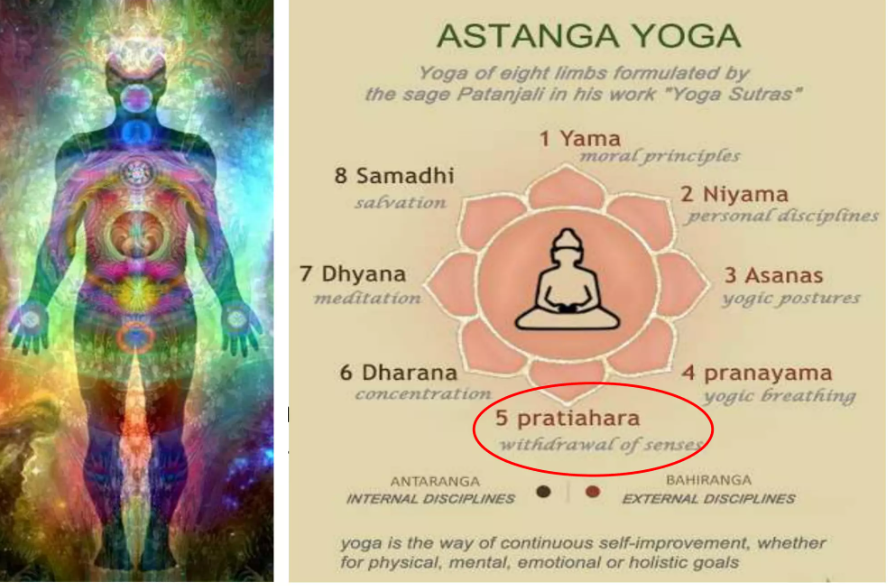
\includegraphics[width=0.6\linewidth,keepaspectratio]{yoganidra2}

		{\tiny (Ref: Yoga Nidra - Dr Amit Chail)}		
        \end{center}

\end{frame}

%%%%%%%%%%%%%%%%%%%%%%%%%%%%%%%%%%%%%%%%%%%%%%%%%%%%%%%%%%%
\begin{frame}[fragile]\frametitle{History}
      \begin{center}
        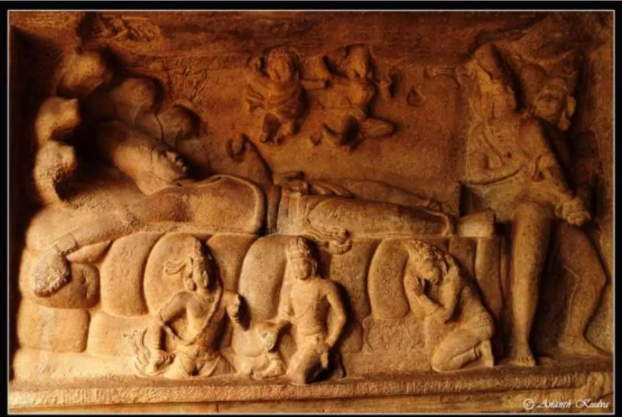
\includegraphics[width=0.8\linewidth,keepaspectratio]{yoganidra3}

		{\tiny (Ref: Yoga Nidra - Dr Amit Chail)}		
        \end{center}

\end{frame}

%%%%%%%%%%%%%%%%%%%%%%%%%%%%%%%%%%%%%%%%%%%%%%%%%%%%%%%%%%%
\begin{frame}[fragile]\frametitle{Four Stages of Human Consciousness}
      \begin{center}
        
\includegraphics[width=0.8\linewidth,keepaspectratio]{yoganidra4}

		{\tiny (Ref: Yoga Nidra - Dr Amit Chail)}		
        \end{center}

\end{frame}

%%%%%%%%%%%%%%%%%%%%%%%%%%%%%%%%%%%%%%%%%%%%%%%%%%%%%%%%%%%
\begin{frame}[fragile]\frametitle{Brain Wave States in Yoga Nidra}
    \begin{itemize}
        \item During Yoga Nidra, consciousness fluctuates between:
        \begin{itemize}
            \item Introversion and extroversion states
            \item Alpha and theta wave states
        \end{itemize}
        \item \textbf{The Nidra State:}
        \begin{itemize}
            \item Located at border between alpha and theta waves
            \item Mind becomes highly receptive
            \item Allows contact with subconscious and unconscious dimensions
            \item Access to dormant potential and hidden solutions
        \end{itemize}
    \end{itemize}
\end{frame}

%%%%%%%%%%%%%%%%%%%%%%%%%%%%%%%%%%%%%%%%%%%%%%%%%%%%%%%%%%%
\begin{frame}[fragile]\frametitle{Practitioners}
      \begin{center}
        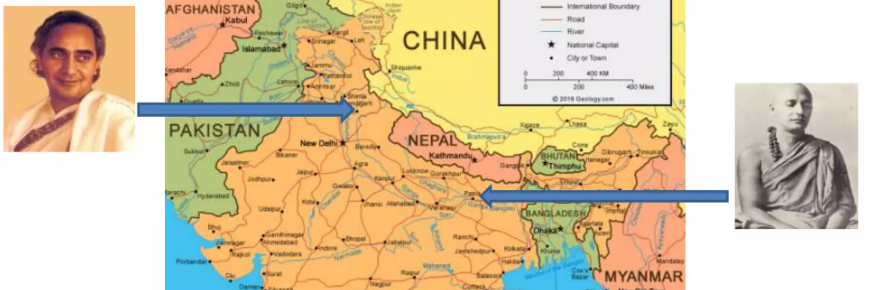
\includegraphics[width=\linewidth,keepaspectratio]{yoganidra5}

		{\tiny (Ref: Yoga Nidra - Dr Amit Chail)}		
        \end{center}

\end{frame}

%%%%%%%%%%%%%%%%%%%%%%%%%%%%%%%%%%%%%%%%%%%%%%%%%%%%%%%%%%%
\begin{frame}[fragile]\frametitle{Modern Development}
    \textbf{Swami Satyananda Saraswati's Contributions:}
    \begin{itemize}
        \item Systematized Yoga Nidra in the 20th century
        \item Founded Bihar School of Yoga
        \item Made the practice accessible to modern practitioners
        \item Emphasized scientific approach to traditional practice
        \item Developed structured methodology for teaching
    \end{itemize}
\end{frame}

%%%%%%%%%%%%%%%%%%%%%%%%%%%%%%%%%%%%%%%%%%%%%%%%%%%%%%%%%%%
\begin{frame}[fragile]\frametitle{Research}
      \begin{center}
        
\includegraphics[width=\linewidth,keepaspectratio]{yoganidra6}

		{\tiny (Ref: Yoga Nidra - Dr Amit Chail)}		
        \end{center}

\end{frame}

%%%%%%%%%%%%%%%%%%%%%%%%%%%%%%%%%%%%%%%%%%%%%%%%%%%%%%%%%%%%%%%%%%%%%%%%%%%%%%%%%%
\begin{frame}[fragile]\frametitle{Sleep vs Yoga Nidra}
    \begin{columns}
        \begin{column}{0.48\textwidth}
            \textbf{Sleep:}
            \begin{itemize}
                \item Unconscious state
                \item No awareness
                \item Natural occurrence
                \item Brain in delta waves
            \end{itemize}
        \end{column}
        \begin{column}{0.48\textwidth}
            \textbf{Yoga Nidra (योगनिद्रा):}
            \begin{itemize}
                \item Conscious relaxation
                \item Maintained awareness
                \item Guided practice
                \item Brain transitions through various wave states
                \item One hour equals 4 hours of regular sleep
            \end{itemize}
        \end{column}
    \end{columns}
\end{frame}

% %%%%%%%%%%%%%%%%%%%%%%%%%%%%%%%%%%%%%%%%%%%%%%%%%%%%%%%%%%%%%%%%%%%%%%%%%%%%%%%%%%
% \begin{frame}[fragile]\frametitle{Nidra vs Yoganidra}
    % \textbf{Nidra (निद्रा)}: \\
    % \begin{itemize}
        % \item Unaware, only physical relaxation.
        % \item Unconscious state.
    % \end{itemize}
    % \vspace{5mm}
    % \textbf{Yoganidra (योगनिद्रा)}: \\
    % \begin{itemize}
        % \item Aware relaxation (physical, mental, and emotional).
        % \item Conscious of subconscious mind.
    % \end{itemize}
% \end{frame}

%%%%%%%%%%%%%%%%%%%%%%%%%%%%%%%%%%%%%%%%%%%%%%%%%%%%%%%%%%%%%%%%%%%%%%%%%%%%%%%%%%
\begin{frame}[fragile]\frametitle{Meditation vs Yoganidra}
    \begin{columns}
        \begin{column}{0.48\textwidth}
            \textbf{Meditation:}
            \begin{itemize}
                \item Typically done sitting up
                \item Focuses on one point of concentration
                \item Requires active mental effort
                \item May be challenging for beginners
            \end{itemize}
        \end{column}
        \begin{column}{0.48\textwidth}
            \textbf{Yoga Nidra (योगनिद्रा):}
            \begin{itemize}
                \item Done lying down
                \item Systematic rotation of awareness
                \item Guided relaxation practice
                \item Accessible to all skill levels
            \end{itemize}
        \end{column}
    \end{columns}
\end{frame}

%%%%%%%%%%%%%%%%%%%%%%%%%%%%%%%%%%%%%%%%%%%%%%%%%%%%%%%%%%%
\begin{frame}[fragile]\frametitle{Science: ECG}
      \begin{center}
        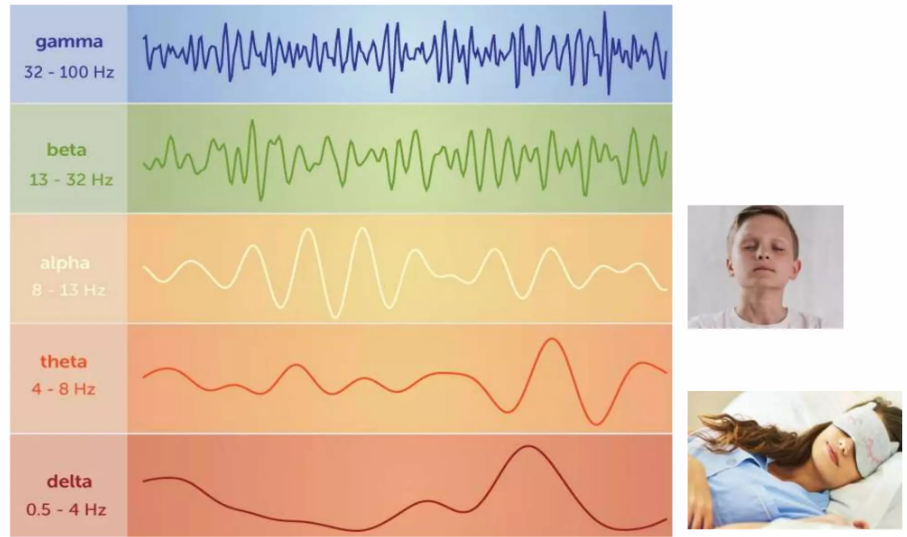
\includegraphics[width=\linewidth,keepaspectratio]{yoganidra9}

		{\tiny (Ref: Yoga Nidra - Dr Amit Chail)}		
        \end{center}

\end{frame}

%%%%%%%%%%%%%%%%%%%%%%%%%%%%%%%%%%%%%%%%%%%%%%%%%%%%%%%%%%%
\begin{frame}[fragile]\frametitle{Science: ECG}
      \begin{center}
        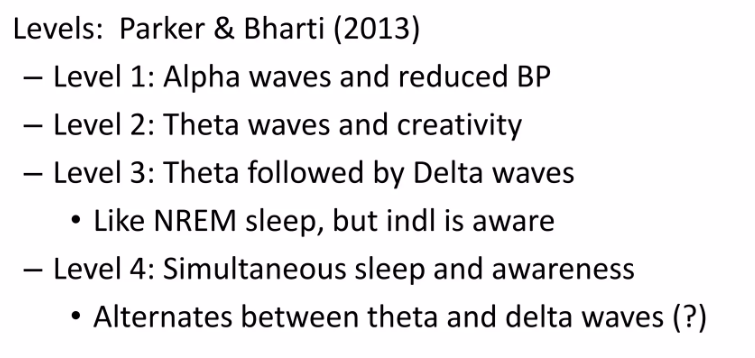
\includegraphics[width=0.8\linewidth,keepaspectratio]{yoganidra10}

		{\tiny (Ref: Yoga Nidra - Dr Amit Chail)}		
        \end{center}

\end{frame}



%%%%%%%%%%%%%%%%%%%%%%%%%%%%%%%%%%%%%%%%%%%%%%%%%%%%%%%%%%%%%%%%%%%%%%%%%%%%%%%%%%
\begin{frame}[fragile]\frametitle{8 Stages of Yoganidra}
    \begin{enumerate}
        \item \textbf{Preparation (Shavasana)}: Deep breaths in Shavasana (शवासन).
        \item \textbf{Resolve (Sankalpa)}: Optional positive affirmation (संकल्प).
        \item \textbf{Body Awareness (Rotation)}: Relax body parts.
        \item \textbf{Breath Awareness}: Relaxation through breath.
        \item \textbf{Opposite Sensations}: Experience and release emotions.
        \item \textbf{Visualization}: Reach the subconscious with imagery.
        \item \textbf{Resolve (Sankalpa)}: Repeat the Sankalpa again.
        \item \textbf{Exiting}: Return awareness to external surroundings.
    \end{enumerate}
\end{frame}

%%%%%%%%%%%%%%%%%%%%%%%%%%%%%%%%%%%%%%%%%%%%%%%%%%%%%%%%%%%%%%%%%%%%%%%%%%%%%%%%%%
\begin{frame}[fragile]\frametitle{Key Instructions}
    \begin{itemize}
        \item No movement during Yoganidra.
        \item Stay awake, do not fall asleep.
        \item Do not think, just follow the instructions.
    \end{itemize}
\end{frame}


%%%%%%%%%%%%%%%%%%%%%%%%%%%%%%%%%%%%%%%%%%%%%%%%%%%%%%%%%%%%%%%%%%%%%%%%%%%%%%%%%%
\begin{frame}[fragile]\frametitle{The Koshas (कोश)}
    \begin{itemize}
        \item \textbf{Annamaya Kosha (अन्नमयकोश)} - Physical Body
        \item \textbf{Pranamaya Kosha (प्राणमयकोश)} - Energy Body
        \item \textbf{Manomaya Kosha (मनोमयकोश)} - Emotional Body
        \item \textbf{Vijnanamaya Kosha (विज्ञानमयकोश)} - Wisdom Body
        \item \textbf{Anandamaya Kosha (आनन्दमयकोश)} - Bliss Body
    \end{itemize}
\end{frame}

%%%%%%%%%%%%%%%%%%%%%%%%%%%%%%%%%%%%%%%%%%%%%%%%%%%%%%%%%%%%%%%%%%%%%%%%%%%%%%%%%%
\begin{frame}[fragile]\frametitle{Koshas in Yoganidra}
    
    \begin{itemize}
        \item Body Awareness (Rotation): \textbf{Annamayakosha (अन्नमयकोश) - Physical Body:} Focus on different body parts (right palm, right arm, legs, back, etc.).
        \item Breath Awareness: \textbf{Pranamayakosha (प्राणमयकोश) - Breath Awareness:} Reverse breath count from 27.
        \item Opposite Sensations: \textbf{Manomayakosha (मनोमयकोश) - Emotional Body:} Experience opposite sensations (hot/cold, wet/dry).
        \item Visualization: \textbf{Vijnanamayakosha (विज्ञानमयकोश) - Subconscious Visualization:} Visualize calming scenes like deserts, lakes, and waves.
    \end{itemize}
\end{frame}

%%%%%%%%%%%%%%%%%%%%%%%%%%%%%%%%%%%%%%%%%%%%%%%%%%%%%%%%%%%%%%%%%%%%%%%%%%%%%%%%%%
\begin{frame}[fragile]\frametitle{Tips for Practicing Yoganidra}
    \begin{itemize}
        \item Use simple and precise language in the script.
        \item Speak in a clear and even tone.
        \item Sit comfortably and be still during facilitation.
        \item Practice in a warm, comfortable space. Use props (pillows, blankets) to support the body.
        \item Remain still, but do not fall asleep.
    \end{itemize}
\end{frame}

%%%%%%%%%%%%%%%%%%%%%%%%%%%%%%%%%%%%%%%%%%%%%%%%%%%%%%%%%%%
\begin{frame}[fragile]\frametitle{Important Considerations}
    \begin{itemize}
        \item \textbf{Consult Healthcare Provider if:}
        \begin{itemize}
            \item Pregnant or recently post-partum
            \item Have serious medical conditions
            \item Experiencing severe mental health issues
        \end{itemize}
        \item \textbf{Practice Guidelines:}
        \begin{itemize}
            \item Avoid practice immediately after meals
            \item Ensure comfortable room temperature
            \item Practice at consistent times
            \item Stay awake during the practice
        \end{itemize}
    \end{itemize}
\end{frame}

\section[Instructs]{Instructions}
%%%%%%%%%%%%%%%%%%%%%%%%%%%%%%%%%%%%%%%%%%%%%%%%%%%%%%%%%%%%%%%%%%%%%%%%%%%%%%%%%%
\begin{frame}[fragile]\frametitle{}
\begin{center}
{\Large Instructions}
\end{center}
\end{frame}

%%%%%%%%%%%%%%%%%%%%%%%%%%%%%%%%%%%%%%%%%%%%%%%%%%%%%%%%%%%%%%%%%%%%%%%%%%%%%%%%%%
\begin{frame}[fragile]\frametitle{Setting Up the Environment}
    \begin{itemize}
        \item \textbf{Room Requirements:}
        \begin{itemize}
            \item Quiet, peaceful space
            \item Comfortable temperature
            \item Dim lighting
            \item No distractions (phone on silent)
        \end{itemize}
        \item \textbf{Best Practice Times:}
        \begin{itemize}
            \item Not immediately after meals
            \item Early morning or before bed
            \item Consistent practice time
        \end{itemize}
    \end{itemize}
\end{frame}

%%%%%%%%%%%%%%%%%%%%%%%%%%%%%%%%%%%%%%%%%%%%%%%%%%%%%%%%%%%%%%%%%%%%%%%%%%%%%%%%%%
\begin{frame}[fragile]\frametitle{Props and Session Duration}
    \begin{itemize}
        \item \textbf{Recommended Props:}
        \begin{itemize}
            \item Yoga mat or comfortable surface
            \item Bolster or pillow under knees
            \item Blanket for warmth
            \item Eye pillow (optional)
        \end{itemize}
        \item \textbf{Session Duration:}
        \begin{itemize}
            \item Beginners: 20-30 minutes
            \item Experienced: Up to 60 minutes
            \item Regular practice: 1-3 times per week
        \end{itemize}
    \end{itemize}
\end{frame}

%%%%%%%%%%%%%%%%%%%%%%%%%%%%%%%%%%%%%%%%%%%%%%%%%%%%%%%%%%%%%%%%%%%%%%%%%%%%%%%%%%
\begin{frame}[fragile]\frametitle{Preparation}
    \begin{itemize}
        \item Lie in Shavasana (शवासन).
        \item Bring your awareness to the space between your body and the earth.
        \item Let your body soften and sink into the floor.    
	\end{itemize}
	
      \begin{center}
        
\includegraphics[width=0.8\linewidth,keepaspectratio]{yoganidra7}

		{\tiny (Ref: Yoga Nidra - Dr Amit Chail)}		
        \end{center}	
\end{frame}

%%%%%%%%%%%%%%%%%%%%%%%%%%%%%%%%%%%%%%%%%%%%%%%%%%%%%%%%%%%%%%%%%%%%%%%%%%%%%%%%%%
\begin{frame}[fragile]\frametitle{Setting the Sankalpa (संकल्प)}
    \begin{itemize}
        \item A positive “I am” statement to guide your Yoganidra practice.
        \item Examples:
        \begin{itemize}
            \item "I am strong."
            \item "I am peaceful."
            \item "I am the witness."
        \end{itemize}
        \item Repeat the Sankalpa 3 times at the start and end of Yoganidra.
    \end{itemize}
\end{frame}

%%%%%%%%%%%%%%%%%%%%%%%%%%%%%%%%%%%%%%%%%%%%%%%%%%%%%%%%%%%%%%%%%%%%%%%%%%%%%%%%%%
\begin{frame}[fragile]\frametitle{Rotation of Awareness (Abbreviated)}
    \textbf{Focus on body parts:}

\begin{columns}
    \begin{column}[T]{0.3\linewidth}
    \begin{itemize}
        \item Right heel
        \item Left heel
        \item Right calf
        \item Left calf
        \item Right knee
        \item Left knee
        \item Right thigh
        \item Left thigh
        \item Both hips
        \item Lower back
        \item Upper back
        \item Right shoulder
        \item Left shoulder
        \item Back of the head
    \end{itemize}

    \end{column}
    \begin{column}[T]{0.7\linewidth}
	      \begin{center}
        
\includegraphics[width=\linewidth,keepaspectratio]{yoganidra8}

		{\tiny (Ref: Yoga Nidra - Dr Amit Chail)}		
        \end{center}
    \end{column}
  \end{columns}
  
  

	
	
\end{frame}

%%%%%%%%%%%%%%%%%%%%%%%%%%%%%%%%%%%%%%%%%%%%%%%%%%%%%%%%%%%%%%%%%%%%%%%%%%%%%%%%%%
\begin{frame}[fragile]\frametitle{Breath Awareness Techniques}
    \textbf{Progressive Breath Work:}
    \begin{itemize}
        \item Place right hand on belly, left hand on chest
        \item Observe natural breath pattern
        \item Make breath bigger gradually:
        \begin{itemize}
            \item Feel belly rise first
            \item Then chest expansion
            \item Hold briefly
            \item Release with gravity
        \end{itemize}
        \item Count breaths backwards from 27
        \item Visualize breath as golden light
    \end{itemize}
\end{frame}

%%%%%%%%%%%%%%%%%%%%%%%%%%%%%%%%%%%%%%%%%%%%%%%%%%%%%%%%%%%%%%%%%%%%%%%%%%%%%%%%%%
\begin{frame}[fragile]\frametitle{Opposite Sensations}
    \begin{itemize}
        \item Bring awareness to the sensation of heat
        \item Feel your whole body becoming warm.
        \item Shift awareness to cold. Feel the entire body cooling down.
        \item Release both sensations.
		\item Similarly: heaviness and lightness, pain and pleasure, love and hate, etc
    \end{itemize}
\end{frame}

%%%%%%%%%%%%%%%%%%%%%%%%%%%%%%%%%%%%%%%%%%%%%%%%%%%%%%%%%%%%%%%%%%%%%%%%%%%%%%%%%%
\begin{frame}[fragile]\frametitle{Guided Imagery}
    \textbf{Journey through Nature:}
    \begin{itemize}
        \item Imagine standing in a meadow, surrounded by a lush forest.
        \item Feel the warmth of the sun and smell the wildflowers.
        \item Walk into the forest, following a path that leads uphill.
        \item Reach a cave and discover a lit candle inside.
        \item Meditate on the candle's flame, with your Sankalpa inscribed on it.
    \end{itemize}
\end{frame}

%%%%%%%%%%%%%%%%%%%%%%%%%%%%%%%%%%%%%%%%%%%%%%%%%%%%%%%%%%%%%%%%%%%%%%%%%%%%%%%%%%
\begin{frame}[fragile]\frametitle{Exiting the Practice}
    \begin{itemize}
        \item Repeat your Sankalpa 3 times.
        \item Bring awareness to the sounds around you.
        \item Slowly move and break Shavasana.
    \end{itemize}
\end{frame}

%%%%%%%%%%%%%%%%%%%%%%%%%%%%%%%%%%%%%%%%%%%%%%%%%%%%%%%%%%%%%%%%%%%%%%%%%%%%%%%%%%
\begin{frame}[fragile]\frametitle{Post-Practice Reflection}
    \textbf{Journaling Guidelines:}
    \begin{itemize}
        \item Record your experience immediately after practice
        \item Note any physical sensations experienced
        \item Document emotional states encountered
        \item Track progress over time
        \item Record any insights or revelations
        \item Compare experiences across different sessions
    \end{itemize}
    \small{This reflection helps deepen your practice and track your progress.}
\end{frame}

%%%%%%%%%%%%%%%%%%%%%%%%%%%%%%%%%%%%%%%%%%%%%%%%%%%%%%%%%%%%%%%%%%%%%%%%%%%%%%%%%%
\begin{frame}[fragile]\frametitle{Best Practices for Teachers}
    \begin{itemize}
        \item \textbf{Voice and Delivery:}
        \begin{itemize}
            \item Speak in a soothing, even tone
            \item Maintain consistent pace
            \item Use clear, simple language
            \item Allow adequate pauses
        \end{itemize}
        \item \textbf{Session Management:}
        \begin{itemize}
            \item Start with shorter sessions (20-30 minutes)
            \item Progress gradually to longer sessions
            \item Always complete all stages
            \item Monitor student comfort
        \end{itemize}
    \end{itemize}
\end{frame}

%%%%%%%%%%%%%%%%%%%%%%%%%%%%%%%%%%%%%%%%%%%%%%%%%%%%%%%%%%%%%%%%%%%%%%%%%%%%%%%%%%
\begin{frame}[fragile]\frametitle{Children's Practice Considerations}
    \begin{itemize}
        \item \textbf{Session Duration:}
        \begin{itemize}
            \item Keep sessions shorter (10-15 minutes)
            \item Use age-appropriate language
            \item Include playful visualization
        \end{itemize}
        \item \textbf{Special Elements:}
        \begin{itemize}
            \item Use simple counting exercises (40 to 1)
            \item Include light visualization exercises
            \item Incorporate gentle encouragement
            \item Allow natural breaks in concentration
        \end{itemize}
        \item \textbf{Closing Practice:}
        \begin{itemize}
            \item End with positive affirmations
            \item Include sharing of "light" with loved ones
            \item Gentle return to regular awareness
        \end{itemize}
    \end{itemize}
\end{frame}

\section[End]{Towards End}
%%%%%%%%%%%%%%%%%%%%%%%%%%%%%%%%%%%%%%%%%%%%%%%%%%%%%%%%%%%%%%%%%%%%%%%%%%%%%%%%%%
\begin{frame}[fragile]\frametitle{}
\begin{center}
{\Large Conclusions}
\end{center}
\end{frame}


%%%%%%%%%%%%%%%%%%%%%%%%%%%%%%%%%%%%%%%%%%%%%%%%%%%%%%%%%%%
\begin{frame}[fragile]\frametitle{Benefits}
      \begin{center}
        
\includegraphics[width=\linewidth,keepaspectratio]{yoganidra11}

		{\tiny (Ref: Yoga Nidra - Dr Amit Chail)}		
        \end{center}

\end{frame}

%%%%%%%%%%%%%%%%%%%%%%%%%%%%%%%%%%%%%%%%%%%%%%%%%%%%%%%%%%%
\begin{frame}[fragile]\frametitle{Benefits}
      \begin{center}
        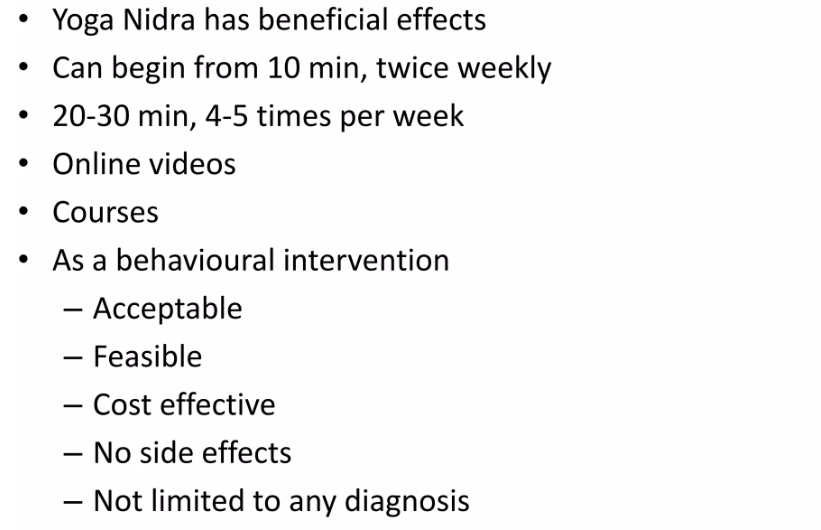
\includegraphics[width=\linewidth,keepaspectratio]{yoganidra12}

		{\tiny (Ref: Yoga Nidra - Dr Amit Chail)}		
        \end{center}

\end{frame}

%%%%%%%%%%%%%%%%%%%%%%%%%%%%%%%%%%%%%%%%%%%%%%%%%%%%%%%%%%%
\begin{frame}[fragile]\frametitle{Summary}
      \begin{center}
        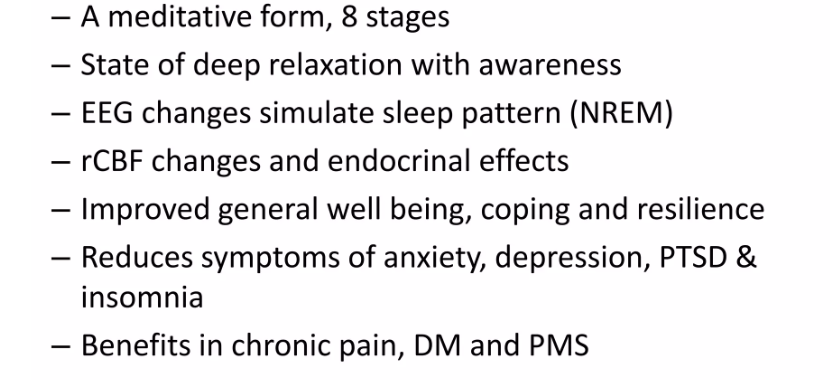
\includegraphics[width=\linewidth,keepaspectratio]{yoganidra13}

		{\tiny (Ref: Yoga Nidra - Dr Amit Chail)}		
        \end{center}

\end{frame}

%%%%%%%%%%%%%%%%%%%%%%%%%%%%%%%%%%%%%%%%%%%%%%%%%%%%%%%%%%%%%%%%%%%%%%%%%%%%%%%%%%
\begin{frame}[fragile]\frametitle{Resources for Further Reading}
    \begin{itemize}
        \item \textbf{Books:}
        \begin{itemize}
            \item "Yoga Nidra" by Swami Satyananda Saraswati.
            \item "Yoga Nidra: A Meditative Practice for Deep Relaxation and Healing" by Richard Miller.
            \item "Yoga Nidra: The Art of Transformational Sleep" by Kamini Desai.
        \end{itemize}
    \end{itemize}
\end{frame}
\end{multicols}

\rule{\linewidth}{0.25pt}
\scriptsize
Copyleft \textcopyleft\  Send suggestions to 
\href{http://www.yogeshkulkarni.com}{yogeshkulkarni@yahoo.com}

\end{document}
